\documentclass[aspectratio=169]{beamer}
\usetheme{Madrid}

\usepackage[utf8]{vietnam}
\usepackage{graphicx}
\usepackage{booktabs}
\usepackage{hyperref}

% Cấu hình thông tin slide
\begin{document}

% ---------------------------------------------
% BÌA (Tùy chỉnh giống báo cáo)
% ---------------------------------------------
\begin{frame}[plain] % Dùng [plain] để bỏ đi header/footer mặc định của Beamer ở trang bìa
    \vspace{-0.5cm} % Cân chỉnh một chút cho vừa chiều cao của slide 16:9
    \begin{center}
        \textbf{\small ĐẠI HỌC QUỐC GIA TP. HỒ CHÍ MINH}\\
        \textbf{\small TRƯỜNG ĐẠI HỌC CÔNG NGHỆ THÔNG TIN}\\[0.1cm]
        
        
\includegraphics[height=1.2cm]{assest/Logo_uit.jpg}\\[0.2cm] % Chỉnh lại height cho phù hợp với slide
        
        \textbf{\large BÁO CÁO ĐỒ ÁN CUỐI KỲ}\\[0.1cm]
        \textbf{\Large MÔN: KỸ NĂNG NGHỀ NGHIỆP}\\[0.1cm]
        \textbf{\small MÃ LỚP: SS004.F31.CN1.CNTT}\\[0.1cm]
        \textbf{\small NHÓM: 02}\\[0.2cm]
        
        \rule{0.8\textwidth}{1pt}\\[0.1cm]
        \textbf{\Large ĐỀ TÀI: XÂY DỰNG VÀ PHÁT TRIỂN}\\[0.1cm]
        \textbf{\Large TRÒ CHƠI TETRIS (XẾP GẠCH)}\\
        \rule{0.8\textwidth}{1pt}
    \end{center}
\end{frame}

% ---------------------------------------------
% GIỚI THIỆU NHÓM & LỚP
% ---------------------------------------------
\begin{frame}{Giới thiệu Thông tin Lớp và Nhóm thực hiện}
    \textbf{Thông tin học phần:}
    \begin{itemize}
        \item \textbf{Môn học:} Kỹ năng nghề nghiệp
        \item \textbf{Mã lớp:} SS004.F31.CN1.CNTT
        \item \textbf{Giảng viên hướng dẫn:} ThS. Nguyễn Văn Toàn % Bạn có thể bỏ chữ ThS nếu không đúng học hàm/học vị
    \end{itemize}
    \vspace{0.3cm}
    
    \textbf{Danh sách thành viên Nhóm SS004:}
    \begin{table}[]
        \centering
        \begin{tabular}{@{}llc@{}}
        \toprule
        \textbf{Họ và tên} & \textbf{MSSV} & \textbf{Vai trò} \\ \midrule
        Phạm Ngọc Hoàng Long & 26730046 & Nhóm trưởng \\
        Huỳnh Thị Kim Anh & 26730002 & Thành viên \\
        Hoàng Gia Huy & 26730026 & Thành viên \\ 
        Lê Thành Nam & 26730050 & Thành viên \\
        Phạm Mạnh Thiên Phúc & 26730057 & Thành viên \\ \bottomrule
        \end{tabular}
    \end{table}
\end{frame}

% ---------------------------------------------
% 1. CÁC CLASS, MODULE
% ---------------------------------------------
\begin{frame}{1. Cấu trúc Game: Các Module và Class chính}
    \textbf{Ứng dụng console một luồng, sử dụng OOP (C++) chia thành các module:}
    \begin{itemize}
        \item \textbf{Module Vòng lặp \& Điều phối (Game Loop):} Quản lý phiên chơi, kiểm soát tốc độ khung hình (30ms/frame).
        \item \textbf{Module Xử lý đầu vào (Input):} Đọc phím không chặn (\texttt{conio.h}).
        \item \textbf{Module Mô hình \& Logic khối (Tetromino):} Các class kế thừa xử lý 7 loại khối, kiểm tra va chạm và xoay.
        \item \textbf{Module Bảng chơi (Board):} Quản lý ma trận lưới, xử lý xóa dòng và tính điểm.
        \item \textbf{Module Hiển thị (Render):} Vẽ lưới và mã màu ANSI (\texttt{windows.h}), vẽ đè không xóa màn hình.
    \end{itemize}
    \vspace{0.2cm}
    \begin{center}
        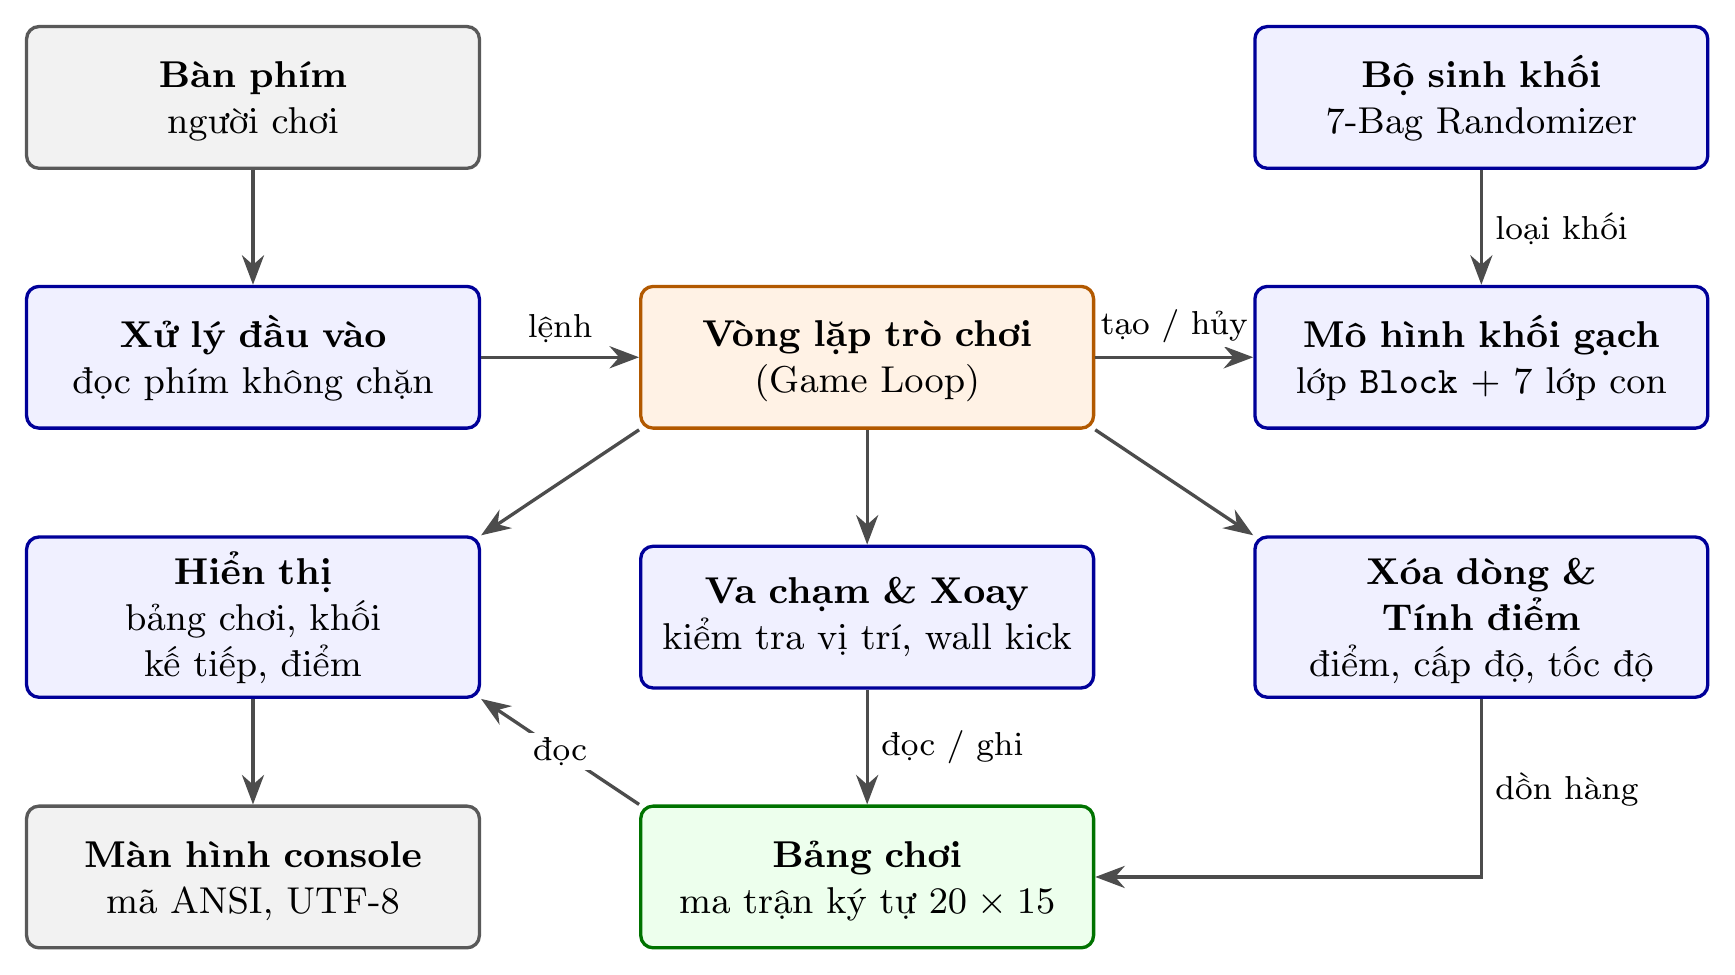
\includegraphics[height=4cm]{04_tai_lieu_ky_thuat/so_do/kien_truc_tong_quan.png}
    \end{center}
\end{frame}

% ---------------------------------------------
% 2. PHÂN CÔNG SV CODE PHẦN NÀO
% ---------------------------------------------
\begin{frame}{2. Phân công Lập trình (Ai code phần nào)}
    \begin{table}[]
        \centering
        \resizebox{\textwidth}{!}{%
        \begin{tabular}{@{}llp{7cm}@{}}
        \toprule
        \textbf{Thành viên} & \textbf{MSSV} & \textbf{Module / Class phụ trách code chính} \\ \midrule
        Phạm Ngọc Hoàng Long & 26730046 & Code \textbf{Module Vòng lặp \& Điều phối}, cấu trúc file \texttt{main.cpp} \\
        Huỳnh Thị Kim Anh & 26730002 & Code \textbf{Module Hiển thị}, xử lý UI và màu sắc ANSI \\
        Hoàng Gia Huy & 26730026 & Code \textbf{Module Mô hình khối (Tetromino)}, xử lý đa hình OOP \\ 
        Lê Thành Nam & 26730050 & Code logic \textbf{Va chạm, Xoay khối} và \textbf{Xử lý Input} \\
        Phạm Mạnh Thiên Phúc & 26730057 & Code \textbf{Module Bảng chơi (Board)}, thuật toán tính điểm \& xóa dòng \\ \bottomrule
        \end{tabular}%
        }
    \end{table}
    \textit{*Ghi chú: Vui lòng sửa lại cột cuối cho khớp chính xác với thực tế của nhóm.}
\end{frame}

% ---------------------------------------------
% 3. CHỨNG MINH GIT - PHẦN 1: PULL REQUEST
% ---------------------------------------------
\begin{frame}{3. Triển khai phân công trên Git: Pull Request}
    \textbf{Minh chứng quy trình làm việc nhóm qua Pull Request trên Git:}
    \begin{itemize}
        \item Mỗi thành viên làm việc trên \textbf{nhánh riêng}, sau đó tạo \textbf{Pull Request} để gộp code vào nhánh chính.
        \item Pull Request giúp cả nhóm \textbf{review code} trước khi merge, tránh lỗi và xung đột.
    \end{itemize}
    \vspace{0.2cm}
    \begin{center}
        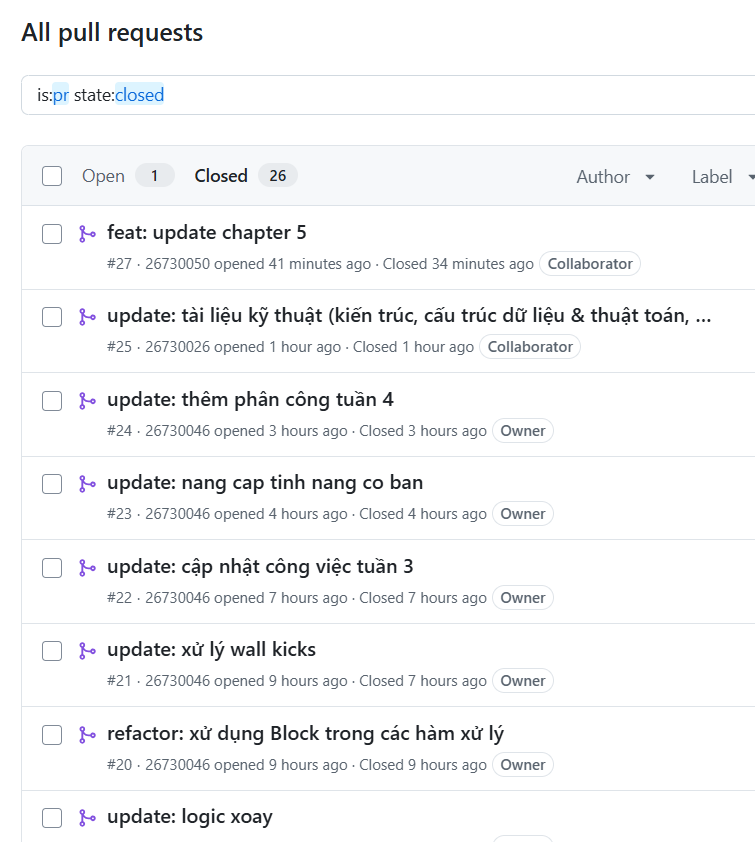
\includegraphics[height=4.5cm]{assest/pull request.png}
    \end{center}
\end{frame}

% ---------------------------------------------
% 4. CHỨNG MINH GIT - PHẦN 2: CONFLICT
% ---------------------------------------------
\begin{frame}{4. Triển khai trên Git: Giải quyết Merge Conflict}
    \begin{columns}
        \begin{column}{0.42\textwidth}
            \textbf{Tình huống thực tế (commit \texttt{9d07350}):}
            \begin{itemize}
                \item \textbf{File:} \texttt{tetris/main.cpp}, hàm \texttt{draw()}
                \item \textbf{Nguyên nhân:} Nhánh local dùng \texttt{cout << "\textbackslash x1B[H"} (ANSI escape), nhánh remote dùng \texttt{SetConsoleCursorPosition} (Windows API).
                \item \textbf{Giải pháp:} Giữ lại \texttt{SetConsoleCursorPosition} để tương thích Windows tốt hơn, rồi \texttt{git add \& commit}.
            \end{itemize}
        \end{column}
        \begin{column}{0.56\textwidth}
            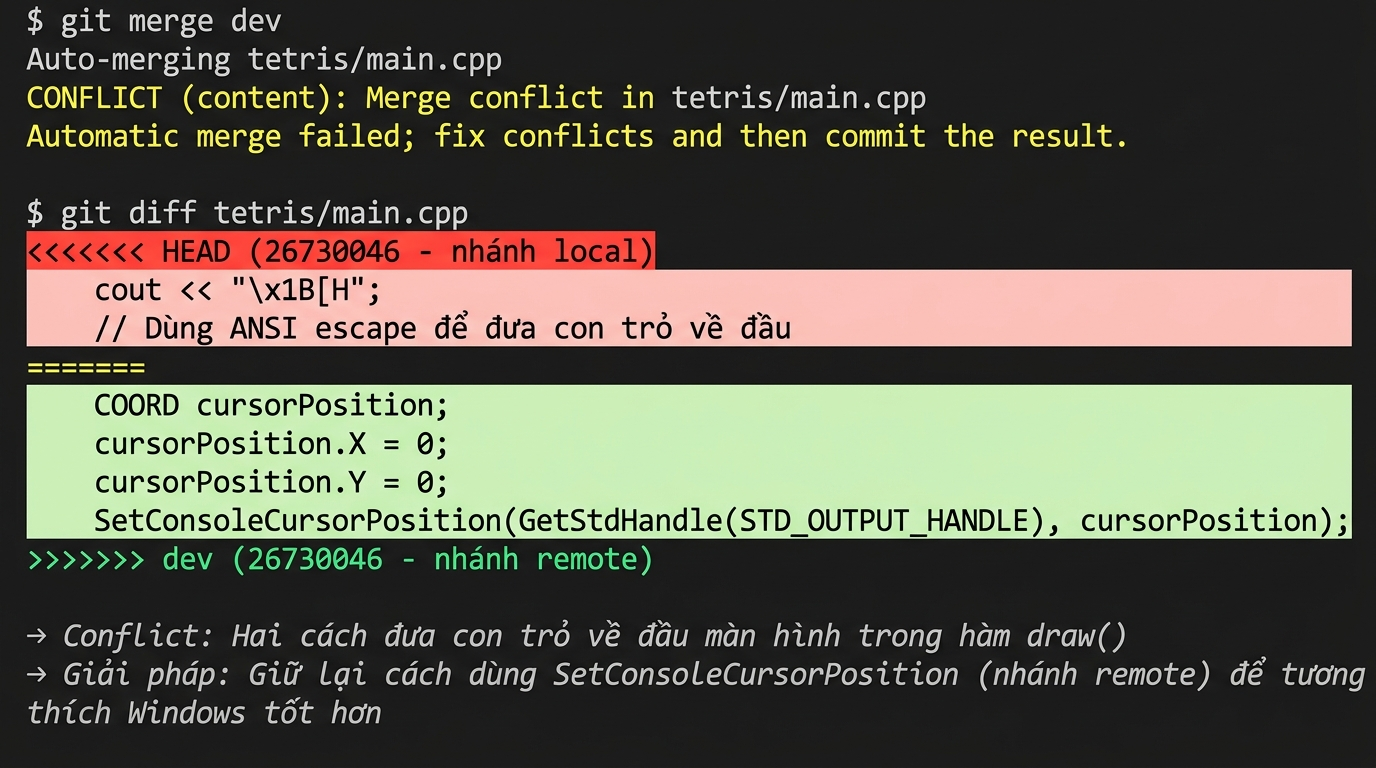
\includegraphics[width=\textwidth]{assest/git_conflict.jpg}
        \end{column}
    \end{columns}
\end{frame}

% ---------------------------------------------
% KẾT THÚC
% ---------------------------------------------
\begin{frame}
    \centering
    \Huge \textbf{Cảm ơn Thầy/Cô đã lắng nghe!}\\
    \vspace{1cm}
    \Large Nhóm rất mong nhận được câu hỏi từ Thầy/Cô.
\end{frame}

\end{document}
